\pgfplotsset{width=\textwidth,compat=1.3}
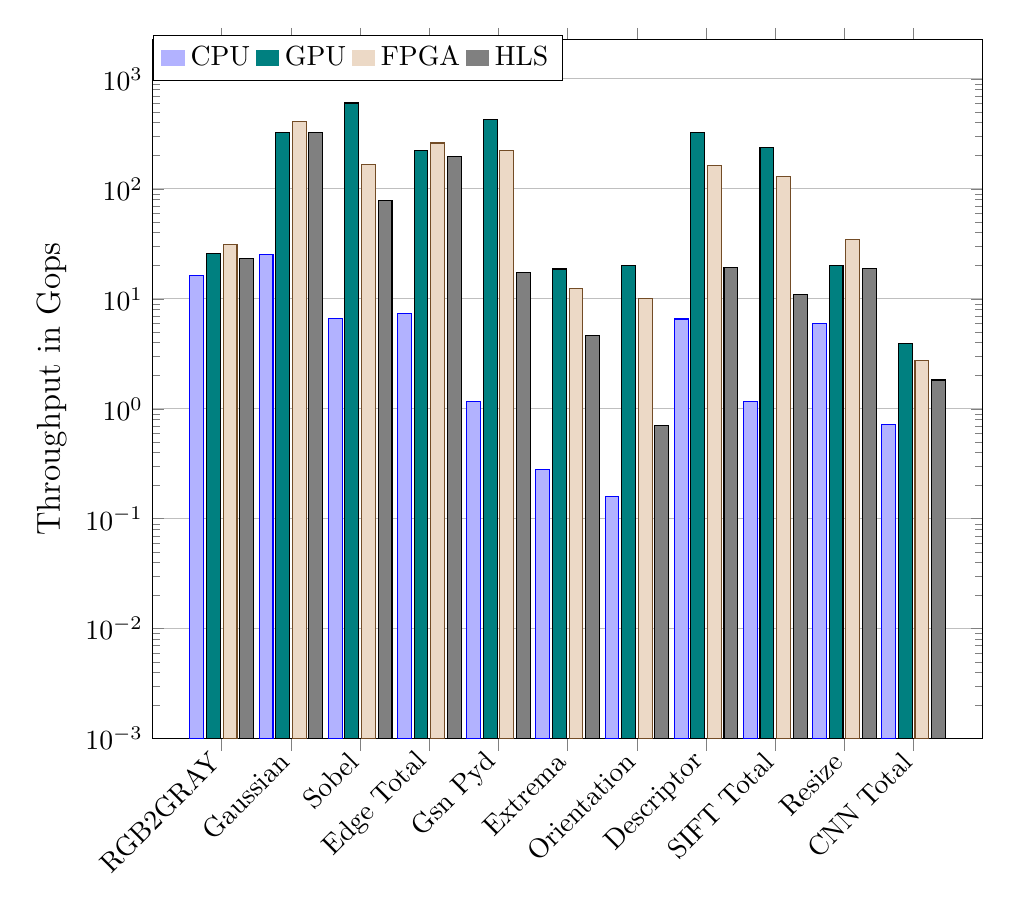
\begin{tikzpicture}
\begin{axis}[
    legend style={},
    ybar=1pt,
    bar width =5pt,
    ymin=0.001,ymax=600,
    enlarge y limits={upper=0.15},
    legend image code/.code={\draw[#1, draw=none] (0cm,-0.1cm) rectangle (0.3cm,0.1cm);
                },
    ymajorgrids = true,
    ymode=log,
    legend style={at={(-0.00000009,0.974)},
                   anchor=west,legend columns=-1},
    ylabel={Throughput in Gops},
    ylabel style={font=\large}, % Adjust the font size of the y-axis label
    symbolic x coords={RGB2GRAY,Gaussian,Sobel,Edge Total,Gsn Pyd,Extrema,Orientation,Descriptor,SIFT Total,Resize,CNN Total},
    xtick=data,
    %nodes near coords,
    nodes near coords style={ anchor=west,rotate=90,inner xsep=0.5pt},
    x tick label style = { rotate=45, anchor=east},
    ]

\addplot coordinates {(RGB2GRAY,16.16) (Gaussian,25.40)  (Sobel,6.60) (Edge Total, 7.29) (Gsn Pyd,1.16) (Extrema,0.28) (Orientation,0.16) (Descriptor,6.55) (SIFT Total,1.17) (Resize,5.92) (CNN Total,0.72)};%CPU

\addplot [fill=teal!]  coordinates {(RGB2GRAY,25.92) (Gaussian,327.76)  (Sobel,604.22) (Edge Total, 223.89) (Gsn Pyd,430.79) (Extrema,18.66) (Orientation,20.00) (Descriptor,327.68) (SIFT Total,239.63) (Resize,20.23) (CNN Total,3.93)};%GPU

\addplot coordinates {(RGB2GRAY,31.10) (Gaussian,406.43)  (Sobel,166.16) (Edge Total, 261.20) (Gsn Pyd,223.88) (Extrema,12.44) (Orientation,10.00) (Descriptor,163.84) (SIFT Total,129.02) (Resize,34.56) (CNN Total,2.76)};%FPGA

\addplot coordinates {(RGB2GRAY,23.47) (Gaussian,327.76)  (Sobel,78.81) (Edge Total, 195.90) (Gsn Pyd,17.46) (Extrema,4.67) (Orientation,0.71) (Descriptor,19.28) (SIFT Total,10.96) (Resize,18.85) (CNN Total,1.83)};%HLS

\legend{CPU,GPU,FPGA,HLS}
\end{axis}
\end{tikzpicture}
